\documentclass[11pt]{article}
\usepackage{geometry}                % See geometry.pdf to learn the layout options. There are lots.
\geometry{letterpaper}                   % ... or a4paper or a5paper or ... 
%\geometry{landscape}                % Activate for for rotated page geometry
%\usepackage[parfill]{parskip}    % Activate to begin paragraphs with an empty line rather than an indent
\usepackage{graphicx}
\usepackage{amssymb,amsmath}
\usepackage{epstopdf}
\usepackage{pgf}
\usepackage{pgfpages}
\usepackage{tikz}
\usetikzlibrary{arrows,backgrounds}
\usepgflibrary{shapes}
\DeclareGraphicsRule{.tif}{png}{.png}{`convert #1 `dirname #1`/`basename #1 .tif`.png}
\pagestyle{empty}


\begin{document}

% Wedge Node Numbering
  \begin{center}
    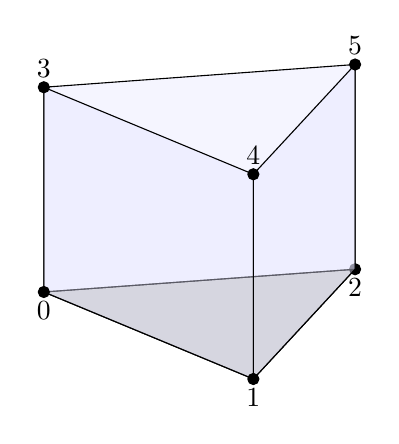
\begin{tikzpicture}[join=round] %Wedge with 6 nodes
        \filldraw[fill=black!20](1.748,.561)--(-2.205,.272)--(.456,-.833)--cycle;
        \filldraw(1.748,.561) circle (2pt);
        \filldraw[fill=blue!10,fill opacity=0.4](-2.205,2.872)--(-2.205,.272)--(1.748,.561)--(1.748,3.161)--cycle;
        \filldraw[fill=blue!10,fill opacity=0.4](1.748,3.161)--(1.748,.561)--(.456,-.833)--(.456,1.767)--cycle;
        \filldraw[fill=blue!10,fill opacity=0.4](.456,1.767)--(.456,-.833)--(-2.205,.272)--(-2.205,2.872)--cycle;
        \filldraw(-2.205,.272) circle (2pt);
        \filldraw(1.748,3.161) circle (2pt);
        \filldraw(-2.205,2.872) circle (2pt);
        \filldraw(.456,-.833) circle (2pt);
        \filldraw(.456,1.767) circle (2pt);
        \fill[black]
                (-2.205,.272) node [below] {0}
                (.456,-.833) node [below] {1}
                (1.748,.561) node [below] {2}
                (-2.205,2.872) node [above] {3}
                (.456,1.767) node [above] {4}
                (1.748,3.161) node [above] {5};
    \end{tikzpicture}
     \hspace{1cm}
     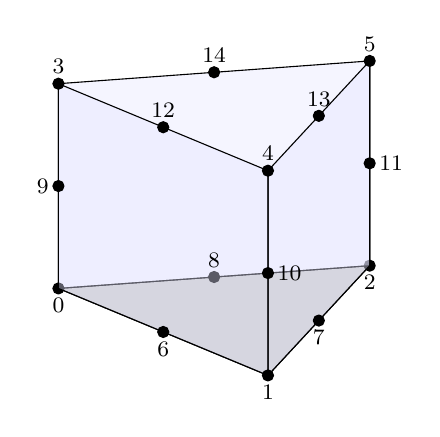
\begin{tikzpicture}[join=round]
         \filldraw[fill=black!20](1.748,.561)--(-2.205,.272)--(.456,-.833)--cycle;
         \filldraw(1.748,.561) circle (2pt);
         \filldraw[fill=blue!10,fill opacity=0.4](-2.205,2.872)--(-2.205,.272)--(1.748,.561)--(1.748,3.161)--cycle;
         \filldraw[fill=blue!10,fill opacity=0.4](1.748,3.161)--(1.748,.561)--(.456,-.833)--(.456,1.767)--cycle;
         \filldraw(-.228,.417) circle (2pt);
         \filldraw(1.748,1.861) circle (2pt);
         \filldraw(-2.205,.272) circle (2pt);
         \filldraw[fill=blue!10,fill opacity=0.4](.456,1.767)--(.456,-.833)--(-2.205,.272)--(-2.205,2.872)--cycle;
         \filldraw(1.748,3.161) circle (2pt);
         \filldraw(-2.205,1.572) circle (2pt);
         \filldraw(-.228,3.017) circle (2pt);
         \filldraw(-2.205,2.872) circle (2pt);
         \filldraw(1.102,-.136) circle (2pt);
         \filldraw(-.874,-.281) circle (2pt);
         \filldraw(1.102,2.464) circle (2pt);
         \filldraw(-.874,2.319) circle (2pt);
         \filldraw(.456,-.833) circle (2pt);
         \filldraw(.456,.467) circle (2pt);
         \filldraw(.456,1.767) circle (2pt);
         \fill[black,font=\footnotesize]
                (-2.205,.272) node [below] {0}
                (.456,-.833) node [below] {1}
                (1.748,.561) node [below] {2}
                (-2.205,2.872) node [above] {3}
                (.456,1.767) node [above] {4}
                (1.748,3.161) node [above] {5}
                (-.874,-.281) node [below] {6}
                (1.102,-.136) node [below] {7}
                (-.228,.417) node [above] {8}
                (-2.205,1.572) node [left] {9}
                (.456,.467) node [right] {10}
                (1.748,1.861) node [right] {11}
                (-.874,2.319) node [above] {12}
                (1.102,2.464) node [above] {13}
                (-.228,3.017) node [above] {14};
    \end{tikzpicture}
  \end{center}
  \begin{center} {(a) \hspace{5cm} (b)} \end{center}
  \begin{center}
    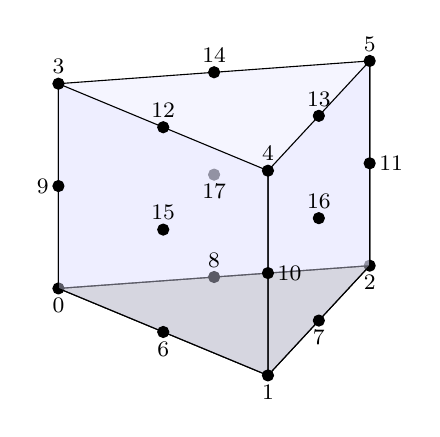
\begin{tikzpicture}[join=round]
        \filldraw[fill=black!20](1.748,.561)--(-2.205,.272)--(.456,-.833)--cycle;
        \filldraw(1.748,.561) circle (2pt);
        \filldraw(-.228,1.717) circle (2pt);
        \filldraw[fill=blue!10,fill opacity=0.4](-2.205,2.872)--(-2.205,.272)--(1.748,.561)--(1.748,3.161)--cycle;
        \filldraw[fill=blue!10,fill opacity=0.4](1.748,3.161)--(1.748,.561)--(.456,-.833)--(.456,1.767)--cycle;
        \filldraw(-.228,.417) circle (2pt);
        \filldraw(1.748,1.861) circle (2pt);
        \filldraw(-2.205,.272) circle (2pt);
        \filldraw[fill=blue!10,fill opacity=0.4](.456,1.767)--(.456,-.833)--(-2.205,.272)--(-2.205,2.872)--cycle;
        \filldraw(1.748,3.161) circle (2pt);
        \filldraw(-2.205,1.572) circle (2pt);
        \filldraw(-.228,3.017) circle (2pt);
        \filldraw(-2.205,2.872) circle (2pt);
        \filldraw(1.102,-.136) circle (2pt);
        \filldraw(-.874,-.281) circle (2pt);
        \filldraw(1.102,1.164) circle (2pt);
        \filldraw(-.874,1.019) circle (2pt);
        \filldraw(1.102,2.464) circle (2pt);
        \filldraw(-.874,2.319) circle (2pt);
        \filldraw(.456,-.833) circle (2pt);
        \filldraw(.456,.467) circle (2pt);
        \filldraw(.456,1.767) circle (2pt);
        \fill[black,font=\footnotesize]
                (-2.205,.272) node [below] {0}
                (.456,-.833) node [below] {1}
                (1.748,.561) node [below] {2}
                (-2.205,2.872) node [above] {3}
                (.456,1.767) node [above] {4}
                (1.748,3.161) node [above] {5}
                (-.874,-.281) node [below] {6}
                (1.102,-.136) node [below] {7}
                (-.228,.417) node [above] {8}
                (-2.205,1.572) node [left] {9}
                (.456,.467) node [right] {10}
                (1.748,1.861) node [right] {11}
                (-.874,2.319) node [above] {12}
                (1.102,2.464) node [above] {13}
                (-.228,3.017) node [above] {14}
                (-.874,1.019) node [above] {15}
                (1.102,1.164) node [above] {16}
                (-.228,1.717) node [below] {17};
    \end{tikzpicture}
  \end{center}
  \begin{center}
           (c) 
  \end{center}
\end{document}  
